\documentclass[a4paper, 10pt]{article}
\usepackage[russian]{babel}
\usepackage[T2A]{fontenc}
\usepackage{geometry}
\usepackage{graphicx}
\usepackage{booktabs}
\geometry{margin=1.5cm}

\begin{document}

\section{Общий пайплайн}

\begin{minipage}[t]{0.5\textwidth}
    \textbf{Raw mri}
    \begin{itemize}
        \item Скачать МРТ снимки T1 weighted, T2 weighted 
        \begin{itemize}
            \item С помощью \texttt{fsl bet} robust brain extraction убрать кости черепа
            \item С помощью \texttt{fsl fast} segmentation выделить серое вещество
            \item С помощью \texttt{fsl flirt} привести МРТ к стандартному пространству MNI152
            \item С помощью \texttt{fsl math} добавить немного гауссовского размытия для сглаживания
        \end{itemize}
    \end{itemize}
\end{minipage}
\hfill
\begin{minipage}[t]{0.4\textwidth}
    \textbf{Preprocessed mri}
    \begin{itemize}
        \item Скачать МРТ снимки T1 weighted, T2 weighted 
    \end{itemize}
\end{minipage}

\vspace{1em}
\noindent
\begin{minipage}{\textwidth}
    \textbf{Общий этап}
    \begin{itemize}
        \item Загрузка всех снимков в память с помощью \texttt{nibabel}.
        \item Так как все снимки разных размеров - приводим все снимки к одному размеру(минимальный размер среди всех снимков) с помощью метода resize из библиотеки \texttt{skimage}.
        \item С помощью алгоритма MPCA понижаем размерность всех снимков: $(N, W, H, D) \rightarrow (N, 3, H, D)$ - аксиальная плоскость.
        \item С помощью алгоритма MPCA понижаем размерность всех снимков: $(N, W, H, D) \rightarrow (N, W, 3, D)$ - фронтальная плоскость.
        \item С помощью алгоритма MPCA понижаем размерность всех снимков: $(N, W, H, D) \rightarrow (N, W, H, 3)$ - сагитальная плоскость.
        \item Сохраняем полученные снимки как обычные png картинки.
        \item Загружаем все картинки в структуру, которая хранит для одного и того же мрт снимка 3 его плоскости после MPCA.
        \item Фиксируем random seed для воспроизводимости эксперимента.
        \item Разделяем датасет на тренировочную и тестовую выборки в соотношении 80\% и 20\% соответственно.
        \item К тренировочной выборке на этапе обучения применяем аугментацию: случайные повороты на 7 градусов, случайные растяжения, случайные отражения по вертикали и горизонтали, гауссовский шум, гауссовское размытие, случайное изменение контраста, насыщенности и яркости.
        \item Все картинки перед входом в нейросеть приводятся к размеру и статистикам ImageNet (потому что используются предобученные сети на ImageNet).
        \item 3 картинки разных плоскостей одного мрт подаются на вход нейросети, а на выходе вектор вероятностей принадлежности к классу. 
    \end{itemize}
\end{minipage}
\section{Архитектура нейросети}
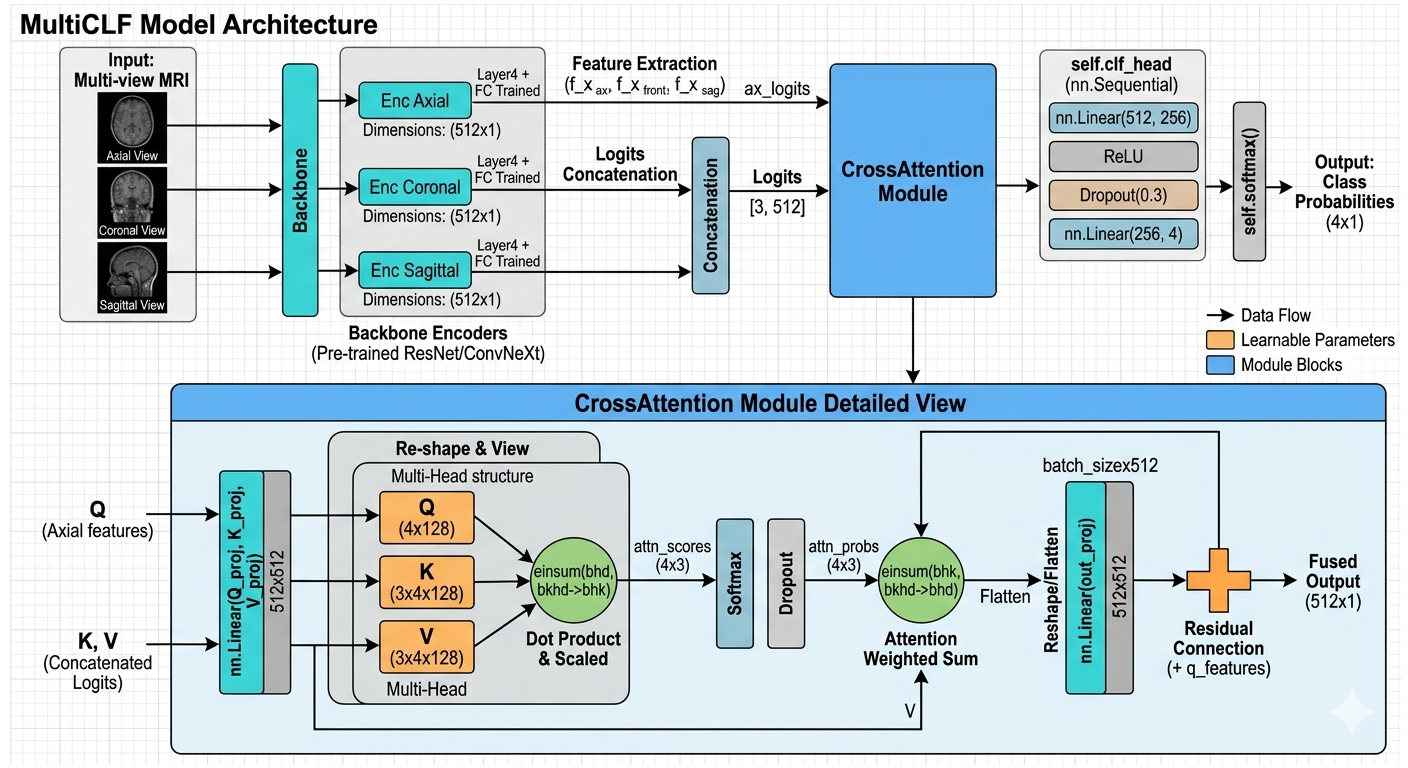
\includegraphics[width=18cm]{arch.png}

\section{Полученные метрики}
\centering
\begin{tabular}{l||c}
    Метрика & Значение \\
    \midrule
    f1 & $0.9505 \pm 0.0400$ \\
    recall & $0.9522 \pm 0.0374$ \\
    precision & $0.9582 \pm 0.0313$ \\
    accuracy & $0.9522 \pm 0.0374$ \\
\end{tabular}
\end{document}